\section{Calibration of electromagnetic objects}
\frame{\tableofcontents[currentsection]}
%%=============================
\begin{frame}{Full calibration}
  To reach the physics analyses, data and simulated reconstructed events must pass a calibration procedure.
  This procedures aim to correct the measured energy to \textcolor{blue}{\bf retrieve the true energy of the particle at the interaction point}.
  \begin{center}
    \begin{tikzpicture}
      \node[anchor=south west] {\includegraphics[width=\linewidth]{ATL-COM-PHYS-2013-1653_1f.pdf}};
%%      \draw[step=1.0,black,thin] (0,0) grid (30,10);
%%      \draw[red, line width=1mm, rounded corners =2pt] ( 20.5, 2.6 ) rectangle ( 24.3, 11 ) ;
      \end{tikzpicture}
  \end{center}
  Electrons and photons follow the same steps but with dedicated analyses. 
%%This analysis continues work from JB Blanchard \& JB de Vivie : \href{https://cds.cern.ch/record/1637533/files/ATL-COM-PHYS-2013-1653.pdf}{\bf ATL-COM-PHYS-2013-1653}.
\end{frame}
%%=============================
%========================
\begin{frame}{MVA calibration}
\begin{itemize}
\item Simulated events are passed through a full GEANT4 simulation of the ATLAS detector.
\item Events are then categorized in $\eta$ and $p_T$ bins, separately for electrons and photons.
\item \textcolor{blue}{\bf A multivariate analysis (MVA) is performed to compute the true energy from detector observables}.
\end{itemize}
Plot shows most probable value (MVP) of $E^{corr}/E^{true}$.
  \begin{minipage}{0.49\linewidth}
    MVA uses :
    \begin{itemize}
    \item Energies in all layers of the ECAL
    \item EM shower shape variables
    \item Barycenters of energy deposits
    \end{itemize}
  \end{minipage}
  \hfill
  \begin{minipage}{0.49\linewidth}
    \includegraphics[width=\linewidth]{CERN-PH-EP-2014-153_2fa.pdf}
  \end{minipage}

\end{frame}
%=================================
\begin{frame}{Energy scale factors}
  \begin{minipage}{0.49\linewidth}
    After MVA calibration, mass distribution of $Z\rightarrow ee$ for data and MC still have \\{\bf discrepancy}.
    \newline
    \textcolor{blue}{\bf A data-driven analysis } is performed to match data to MC distribution \\(relative matching).
  \end{minipage}
  \hfill
  \begin{minipage}{0.49\linewidth}
    \includegraphics[width=\linewidth]{CalibSupNote_Distri_m12_uncorrected.pdf}
  \end{minipage}

A correction, applied to both electrons of Z decay, is computed to shift the central value of data distribution : 
\begin{center} \textcolor{blue}{\bf energy scale factor ($\alpha$)} \end{center}
$$E^{corr}=E^{meas}(1+\alpha)$$
\end{frame}

%%============================
\begin{frame}{Resolution constant term}
  \input{/home/goudet/Documents/LAL/ExternalPlot/ResolutionConstantTerm.tex}
  \begin{itemize}
  \item $a$ : sampling term ( $10\%$). Linked to the fluctuations of electromagnetic showers. \\Can be simulated.
  \item $b/E$ : noise term ( $350cosh(\eta )$~MeV ). Measured in dedicated runs.
  \item {\bf c : constant term ($0.7\%$)}. Must be measured on data.
  \end{itemize}
  We observe that data distribution is larger than MC. 
  An {\bf additional constant term (C)} is measure to enlarge MC up to the data width.
  Both MC electrons undergo the correction :
  \begin{center}\textcolor{blue}{\bf Resolution constant term (C) }\end{center}
  $$E^{corr} = E^{meas}(1+N(0,1)*C)$$
  $N(0,1)$ : a Gaussian distributed random number
\end{frame}

%%===================================
\begin{frame}{Template method}
\begin{minipage}{0.59\linewidth}
  The template method is used to measure $\alpha$ and $C$ simultaneously.
\begin{itemize}
\item Create distorded MC (templates) with test values of $\alpha$ and $C$.
\item \textcolor{blue}{\bf Compute $\chi^2$ between Z mass distribution of data and template}.
\item \textcolor{blue}{\bf Fit the minimum of the $\chi^2$ distribution} in the ($\alpha,C$) plane.
\item Fit performed in 2 steps of 1D fits : 
\begin{itemize}
\item fit $\chi^2=f(\alpha)$ at constant $C$ (lines) $\rightarrow (\alpha_{min}, \chi^2_{min})$ .
\item fit $\chi^2_{min}=f(C)\rightarrow (C, \Delta C)$
\item project $C$ in $\alpha_{min}=f(C)$, corresponding bin gives $(\alpha, \Delta\alpha)$.
\end{itemize}
\end{itemize}
  \includegraphics[width=0.325\linewidth]{MC6_0_0_chi2FitNonConstVar_10.pdf}
  \includegraphics[width=0.325\linewidth]{MC6_0_0_chi2FitConstVar.pdf}
  \includegraphics[width=0.325\linewidth]{MC6_0_0_corAngle.pdf}
\end{minipage}
\hfill
\begin{minipage}{0.4\linewidth}
  \includegraphics[width=\linewidth]{MC6_0_0_CompareAlpha.pdf}\\
  \includegraphics[width=\linewidth]{MC6_0_0_chiMatrix.pdf}\\
\end{minipage}
\end{frame}

%========================================
\begin{frame}{Detector splitting}
  \begin{minipage}{0.49\linewidth}
    \includegraphics[width=\linewidth]{ATLASCaloPerf_2fi.pdf}
  \end{minipage}
  \begin{minipage}{0.49\linewidth}
    \begin{itemize}
    \item Detector is not uniform along $\eta$.
    \item To improve resolution, \\ \textcolor{blue}{\bf calibration is performed in bin of $\eta_{calo}$.}
    \item 68 and \textcolor{brown}{24} bins are used respectively for $\alpha$ and $C$.\\
      {\tiny \textcolor{brown}{0} 0.1 \textcolor{brown}{0.2} 0.3 \textcolor{brown}{0.4} 0.5 \textcolor{brown}{0.6} 0.7 \textcolor{brown}{0.8} 0.9 \textcolor{brown}{1} 1.1 \textcolor{brown}{1.2} 1.285 \textcolor{brown}{1.37} 1.42 1.47 1.51 \textcolor{brown}{1.55} 1.59 1.63 1.6775 1.725 1.7625 \textcolor{brown}{1.8} 1.9 \textcolor{brown}{2} 2.05 2.1 2.2 \textcolor{brown}{2.3} 2.35 2.4 2.435 \textcolor{brown}{2.47}}
    \end{itemize}
  \end{minipage}
  \vfill
  {\bf Electrons are labelled by their $\eta$ bin}, hence Z are labeled by the combination of electrons bins.
  \textcolor{blue}{\bf Scales are computed for each combination.}
\end{frame}

%============================

\begin{frame}{Inversion Procedure}
Obtaining \textcolor{blue}{\bf electron scales from Z scales} need the minimizations of the following $\chi^2$'s
\begin{equation}
\begin{array}{l}
\chi^2 = \sum \limits_{i, j\leq i} \frac{ (\alpha_i + \alpha_j - 2\alpha_{ij})^2 }{(\Delta\alpha_{ij})^2}\\
\chi^2 = \sum \limits_{i, j\leq i} \frac{ (\sqrt{\frac{c_i^2 + c_j^2}{2}} - c_{ij})^2 }{\Delta^2 c_{ij}}
\end{array}
\end{equation}
\begin{center}
\begin{minipage}{0.40\linewidth}
    \includegraphics[width=\linewidth]{Closure24_alpha.pdf}
\end{minipage}
\begin{minipage}{0.40\linewidth}
    \includegraphics[width=\linewidth]{Closure24_c.pdf}
\end{minipage}
\end{center}
\end{frame}

%%===================================
\begin{frame}{Run 2 results}
  \begin{itemize}
  \item $\alpha$ measured independently for each year.
  \item $c$ measured on combined data.
    \end{itemize}

  \begin{minipage}{0.49\linewidth} 
    \includegraphics[width=\linewidth]{CalibSupNote_CS_alphaOff.pdf}
  \end{minipage}
  \hfill
  \begin{minipage}{0.49\linewidth}
    \includegraphics[width=\linewidth]{CalibSupNote_CS_cOff.pdf}
  \end{minipage}
%  {\bf $\alpha$  discrepancies are below $0.1\%$ } out of the crack ($1.37<|\eta|<1.55$).
\end{frame}
%===============================================
\begin{frame}{Uncertainties}
  12 (13) sources of uncertainties have been evaluated for $\alpha$ ($c$).

    \begin{minipage}{0.49\linewidth} 
      \includegraphics[width=\linewidth]{CalibSupNote_totUncAlpha.pdf}
  \end{minipage}
  \hfill
  \begin{minipage}{0.49\linewidth}
    \includegraphics[width=\linewidth]{CalibSupNote_totUncC.pdf}
  \end{minipage}

  \begin{center}
    \begin{minipage}{0.7\linewidth}
      \centering
      {\bf Main sources }
      \begin{itemize}
      \item Diff. btw tight and medium electrons
      \item Closure
      \item Bremsstrahlung impact on electron momentum
      \end{itemize}
    \end{minipage}
  \end{center}
\end{frame}
%===============================================
\begin{frame}{Runs comparison}
  Performances of run 2 in-situ calibration surpass run 1 results.

  \begin{minipage}{0.42\linewidth} 
    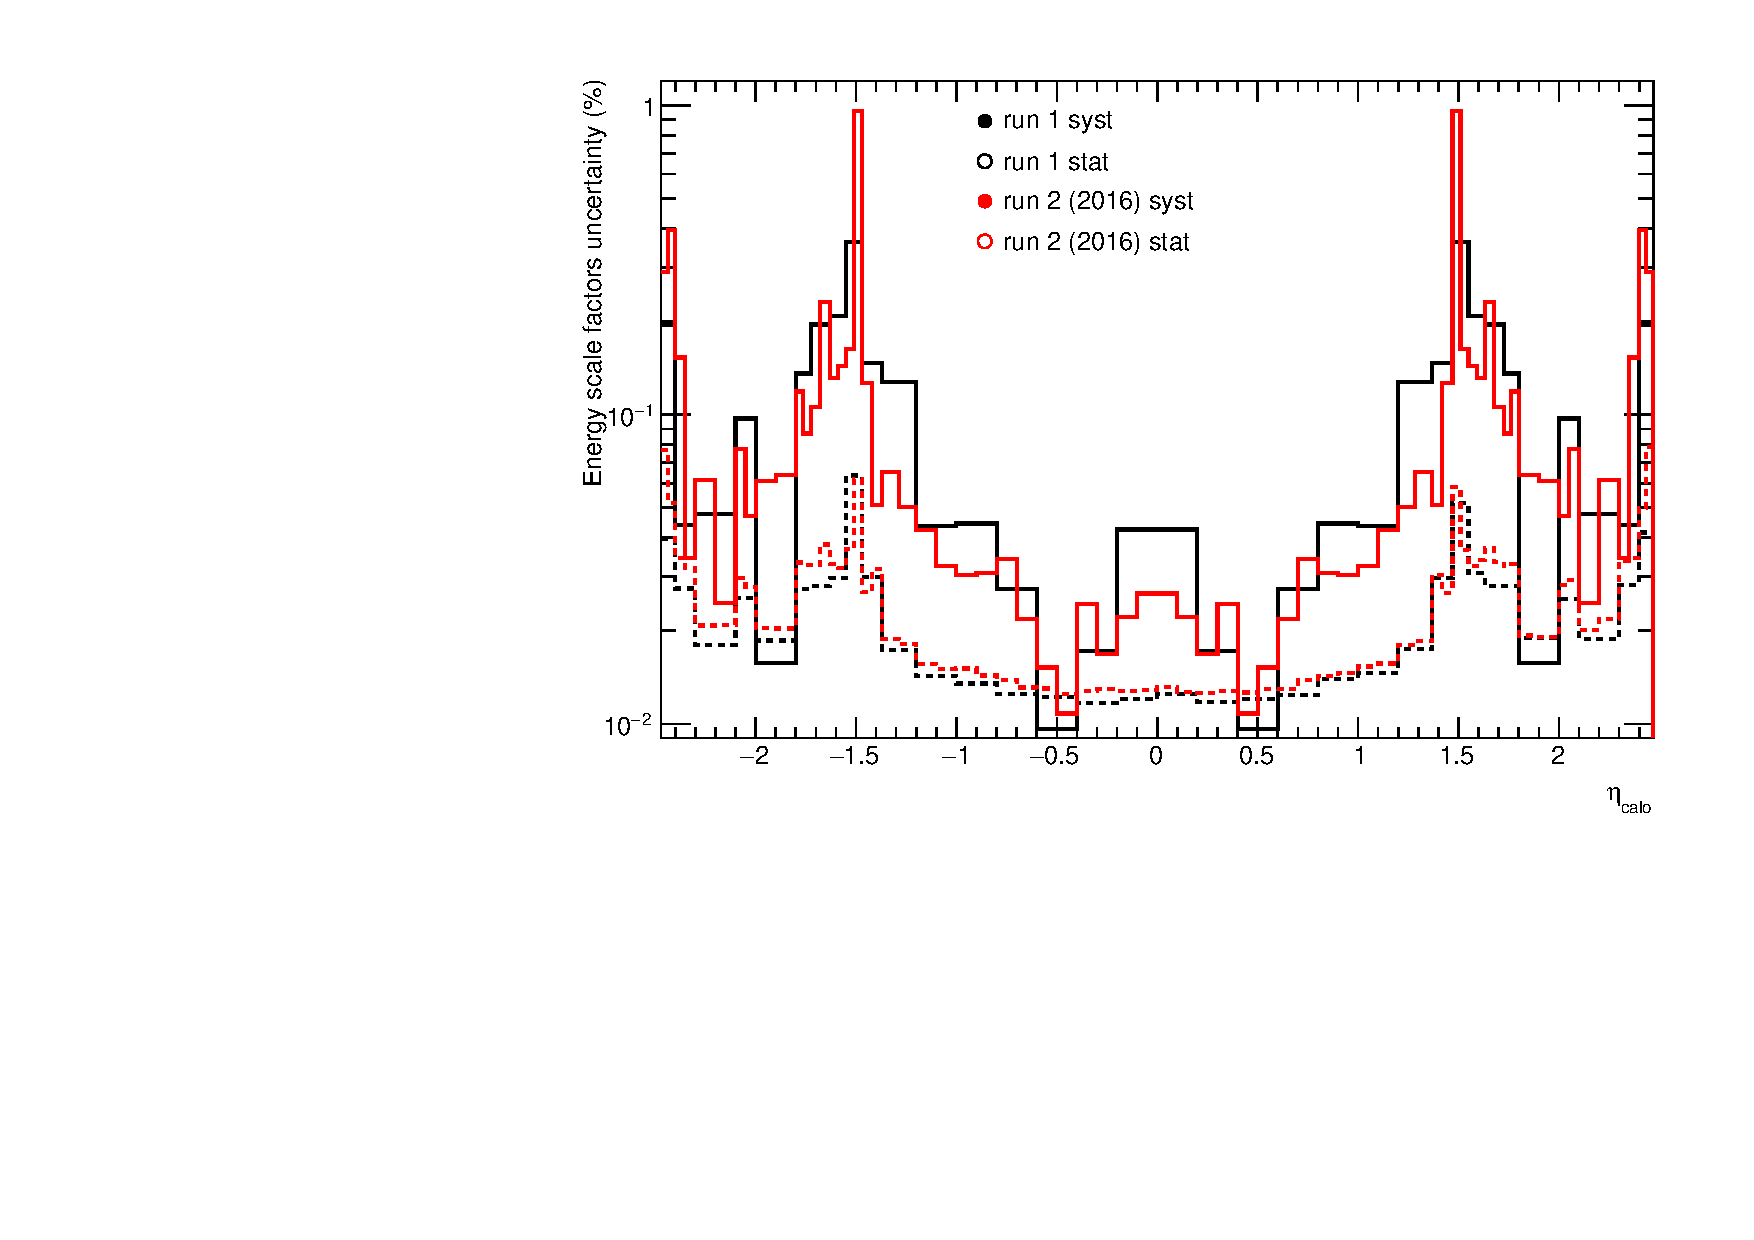
\includegraphics[width=\linewidth]{Figures/CompareSystRun_alpha.pdf}
  \end{minipage}
  \hfill
  \begin{minipage}{0.42\linewidth}
    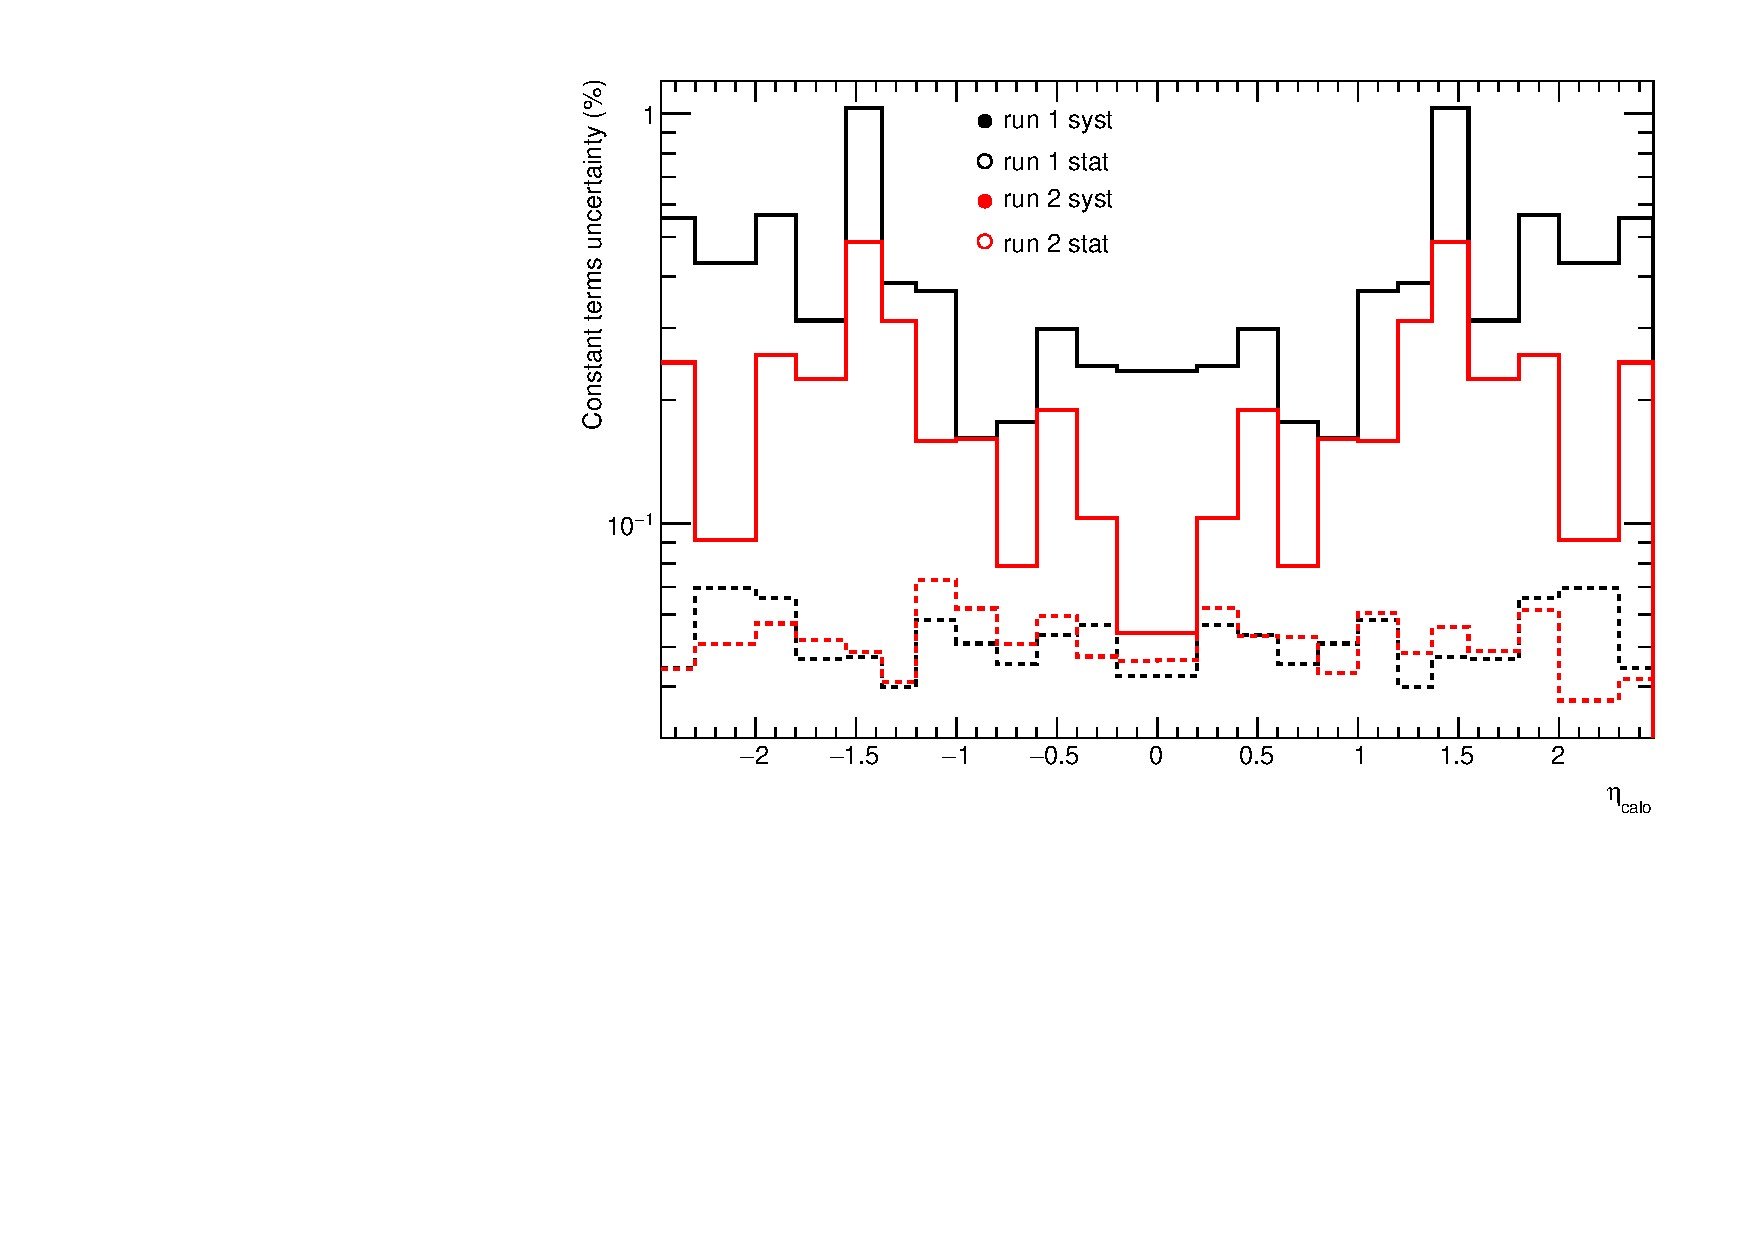
\includegraphics[width=\linewidth]{Figures/CompareSystRun_c.pdf}
  \end{minipage}
  \centering
  \begin{minipage}{0.53\linewidth}
    \includegraphics[width=\linewidth]{CalibSupNote_Distri_m12_corrected.pdf}
  \end{minipage}

\end{frame}

%===========================================
\begin{frame}{Photon correction}
Electrons scale factors are also applied to photons. 
A residual scale factor ($\Delta\alpha$) is measured from $Z\rightarrow ll\gamma$.

No significant deviation observed.
\newline
  \begin{minipage}{0.49\linewidth}
    \includegraphics[width=\linewidth]{CERN-PH-EP-2014-153_34fa.pdf}
  \end{minipage}
  \hfill
  \begin{minipage}{0.49\linewidth}
    \includegraphics[width=\linewidth]{CERN-PH-EP-2014-153_34fb.pdf}
  \end{minipage}
\end{frame}

